\label{s:filtering_haar}
%
%\begin{figure}[t]
\centering
\begin{tabular}{@{}c c@{}} % @{} removes padding around the edge of the table
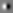
\includegraphics[width=0.2\columnwidth]{\figpath/filtering/Gx} &
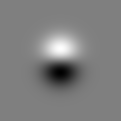
\includegraphics[width=0.2\columnwidth]{\figpath/filtering/Gy} \\
(a) & (b)
\end{tabular}
%
\caption{First derivatives (a) $\Gx$ and (b) $\Gy = \Gx^T$}
\label{f:filters_firstderivs}
\end{figure}%

When using second derivatives, orientation can be computed analytically from the responses, $\Ixy$ and $\Ixx-\Iyy$, to the filters $\Gxy$ and $\Gxx-\Gyy$, respectively. These filters have a distinctive `cloverleaf' appearance that can be approximated by highly efficient Haar-like features that have demonstrated considerable success in applications such as face detection~\cite{Viola_Jones_IJCV04}. To approximate the latter filter, $\Gxx-\Gyy$, we used a modification of the summed area table to compute features at $45^\circ$~\cite{Lienhart_Maydt_ICIP02}.

One downside to this approach is that when using responses to second derivatives (or their Haar-like approximation) we must compute the responses at the two possible solutions to determine which is the correct one. With the Haar-like approximation that combines the response to $\Ixx$ and $\Iyy$, this analytic solution is no longer available and a regression approach becomes necessary.
% i.e. there is no analytic solution when using a Haar-like approximation